\chapter{Resultados e produtos obtidos}

\section{Implementações dos métodos}
  \subsection{Protótipo básico}
  O protótipo básico foi uma prova de conceito bem sucedida para a implementação do método implementação em si e suas limitações, bem como para o uso das linguagens CUDA e OpenCL para este fim.
  
  Sua compilação é bastante simples através do comando \textit{make}. Sem nenhum argumento ele compilará a versão em \textit{C++} por padrão. Com os argumentos \textit{cuda} ou \textit{opencl} serão compiladas suas respectivas versões. Abaixo está o processo de compilação
  
  {\scriptsize
  \begin{verbatim}
$ make cuda
g++ -c -Wall -pedantic -Wextra  -Iinclude main.cpp
g++ -c -Wall -pedantic -Wextra  -Iinclude io/input.cpp
g++ -c -Wall -pedantic -Wextra  -Iinclude core/dataset.cpp
g++ -c -Wall -pedantic -Wextra  -Iinclude core/fiber.cpp
g++ -c -Wall -pedantic -Wextra  -Iinclude io/output.cpp
g++ -c -Wall -pedantic -Wextra  -Iinclude io/gui/primitives/cylinder.cpp
g++ -c -Wall -pedantic -Iinclude io/gui/window_manager.cpp
g++ -c -Wall -pedantic -Wextra  -Iinclude io/gui/scene.cpp
g++ -c -Wall -pedantic -Wextra  -Iinclude io/gui/primitives/cylinder_collection.cpp
g++ -c -Wall -pedantic -Wextra  -Iinclude io/gui/primitives/cone.cpp
g++ -c -Wall -pedantic -Wextra  -Iinclude io/gui/primitives/cone_collection.cpp
nvcc -c -Iinclude core/cuda/rk.cpp -o rk_cuda.o -arch sm_20
nvcc -c -Iinclude core/cuda/rk_kernel.cu -o rk_cuda_kernel.o -arch sm_20
nvcc main.o input.o dataset.o fiber.o output.o cylinder.o window_manager.o scene.o
  cylinder_collection.o cone.o cone_collection.o rk_cuda.o rk_cuda_kernel.o -o rk
  -arch sm_20 -lglut -lGL -lGLU -lm -lpthread -lX11
  \end{verbatim}
  }
  
  \newpage
  Sua interface é bastante básica, mas permite rotacionar o campo e a fibra, transladá-lo, aproximá-lo ou afasta-lo tudo através de teclas. Além disso, é possível escolher quais informações são exibidas. Ou seja, é possível escolher entre exibir ou ocultar o campo vetorial, as fibras resultantes do RK2 ou as fibras resultantes do RK4.
  
  A única limitação encontrada para esta implementação é lidar com a inderteminação que existe no campo vetorial na região de intersecção de duas fibras. Esta indeterminação faz com que o método possa seguir qualquer uma das fibras na intersecção quando chega a esta região.
  
  \begin{figure}[!h]
    \begin{center}
      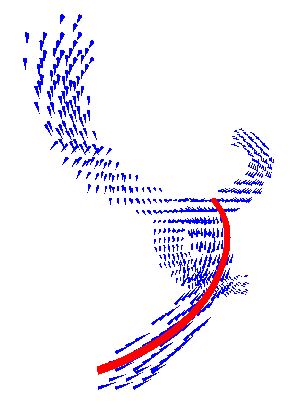
\includegraphics[width=72mm, height=100mm]{images/fibraecampo.png}
      \label{fig:fibraecampo}
      \caption{Campo 32x32x32 com duas hélices. Ao chegar na intersecção, a fibra se desvia para fora do campo e o método entende que terminou de propagá-la devido à baixa intensidade dos vetores.}
    \end{center}
  \end{figure}
  
  Indo além, os testes deste protótipo com ressonâncias reais gerou o mesmo resultado do software de exploração de imagens médicas BioImage Suite (\ref{bioimage}), como podemos observar a seguir.
  
  \begin{figure}[!h]
    \begin{center}
      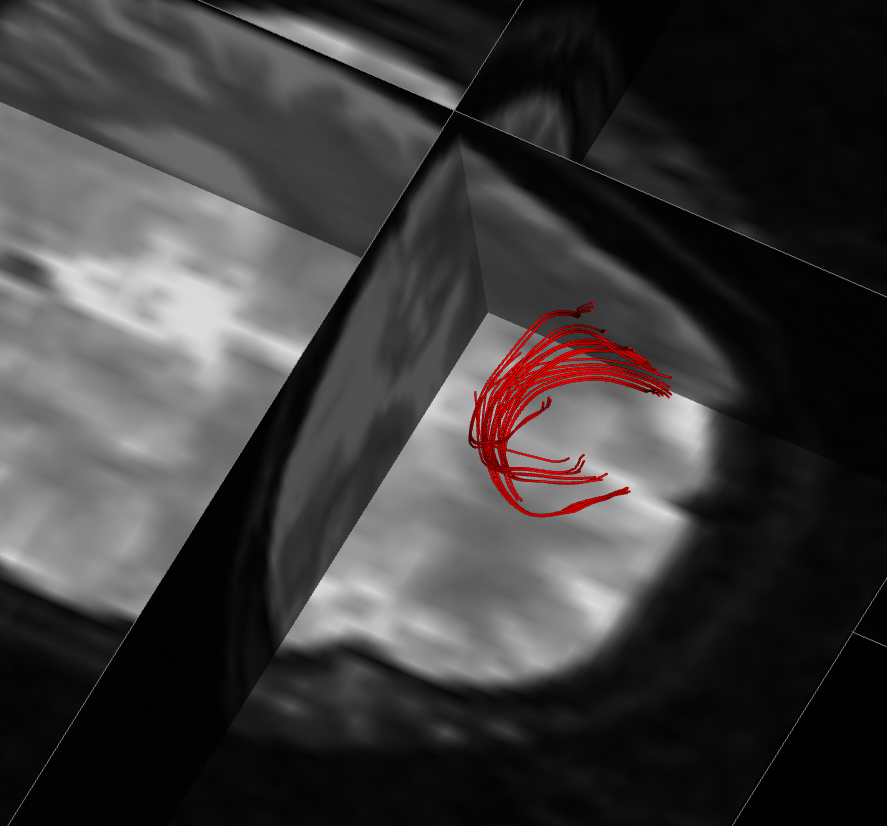
\includegraphics[width=100mm, height=72mm]{images/bioimage-dti.png}
      \label{fig:bioimage-dti}
      \caption{Resultado da tractografia realizada pelo BioImage Suite em uma ressonância magnética.}
    \end{center}
  \end{figure}
  
  \begin{figure}[!h]
    \begin{center}
      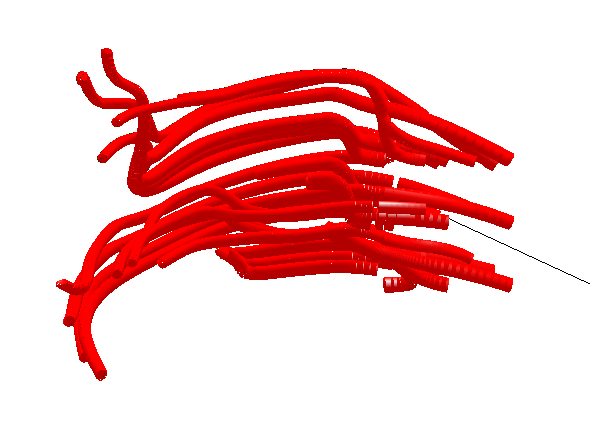
\includegraphics[width=100mm, height=72mm]{images/prototype-dti.png}
      \label{fig:prototype-dti}
      \caption{Resultado da tractografia realizada pelo pelo protótipo na mesma ressonância magnética da figura 4.2.}
    \end{center}
  \end{figure}
  
  Como podemos observar, o resultado (em vermelho) obtido por ambos é o mesmo, confirmando a corretude do protótipo gerado comparando-o a um software já consolidado.
  
  \subsection{Protótipo utilizando a VTK}
  Este protótipo utilizou a versão 5.6 da biblioteca \textit{VTK} para servir como uma prova de que é possível implementar o método dentro da biblioteca, posteriormente sendo útil para o planejamento do que deve ser feito para extende-lo em \textit{GPU} no futuro.
  
  A única dependência que existe, é a instalação da biblioteca \textit{VTK} 5.6. Com isto, sua compilação é ainda mais simples que o protótipo anterior utilizando software de compilação multiplataforma \textit{CMake}. Os resultados de uma compilação bem sucedida podem ser vistos a seguir:
  
  {\scriptsize
  \begin{verbatim}
  $ cmake .
  -- The C compiler identification is GNU 4.7.2
  -- The CXX compiler identification is GNU 4.7.2
  -- Check for working C compiler: /usr/bin/gcc
  -- Check for working C compiler: /usr/bin/gcc -- works
  -- Detecting C compiler ABI info
  -- Detecting C compiler ABI info - done
  -- Check for working CXX compiler: /usr/bin/c++
  -- Check for working CXX compiler: /usr/bin/c++ -- works
  -- Detecting CXX compiler ABI info
  -- Detecting CXX compiler ABI info - done
  -- Configuring done
  -- Generating done
  -- Build files have been written to: ./runge-kutta-vtk
  $ make
  Scanning dependencies of target RungeKutta
  [ 20%] Building CXX object CMakeFiles/RungeKutta.dir/Main.cpp.o
  [ 40%] Building CXX object CMakeFiles/RungeKutta.dir/io/input/Input.cpp.o
  [ 60%] Building CXX object CMakeFiles/RungeKutta.dir/io/input/AnalyzeReader.cpp.o
  [ 80%] Building CXX object CMakeFiles/RungeKutta.dir/core/cpp/Tracer.cpp.o
  [100%] Building CXX object CMakeFiles/RungeKutta.dir/io/output/Renderer.cpp.o
  Linking CXX executable RungeKutta
  [100%] Built target RungeKutta
  \end{verbatim}
  }
  
  Sua interface possui as mesmas funcionalidades que a do protótipo anterior, permitindo rotação, translação e escala. Da mesma forma este protótipo também não é capaz de lidar com indeterminações em um campo vetorial.
  
  \begin{figure}[!h]
    \begin{center}
      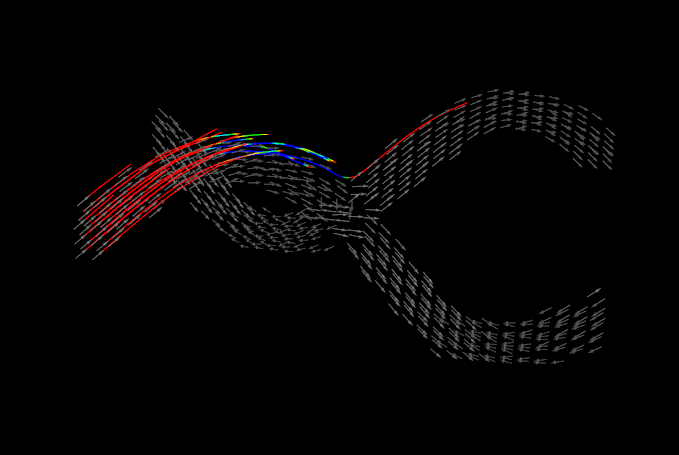
\includegraphics[width=100mm, height=72mm]{images/fibraecampo-vtk.png}
      \label{fig:fibraecampo-vtk}
      \caption{Campo 32x32x32 com duas hélices. Ao chegar na intersecção, a fibra se desvia para um fora do campo e o método entende que terminou de propaga-la devido à baixa intensidade dos vetores ou se desvia para outraq hélice devido à indeterminação do campo na intersecção.}
    \end{center}
  \end{figure}
